\chapter{Time Plan}
Our first meeting was on 7th October 2013. The team met with the supervisor and started 
planning on the same week. The Gantt chart presented in Figure \ref{fig:gantt} to show the 
exact time intervals planned for each stage of the project. This is the most up to date
plan we have at the moment, but please keep in mind that parts of it will be extended 
or updated in the future as the need arises.

\section{Background Research: 07/10/2013 -- 25/10/2013}
All team members will have to do their own research about Minecraft. Everyone should play the game to get more familiar with it and understand its key concepts. We will look up how to create a mod for the game and find tools and resources to do so.
The team will also read the most relevant parts of a thesis suggested by our supervisor. The name of the study is “The Effective Integration of Digital Games and Learning Content" written by Jacob Habgood. 
We must read the ``National Curriculum in England, Key Stage 2'' in order to understand what mathematical elements to include in our game.

\section{Initial Decisions: 14/10/2013 -- 23/10/2013} 
The team will identify the most important activities of the project and choose members to be responsible for different duties. All team members should take the Belbin personality test on-line as suggested by our supervisor. The team will decide on which development tools to be used and what software development methodologies and techniques to be followed. Ideas will be discussed during this period. The team will decide what basic concepts and features the game must have during the early stages of development.

\section{Website \& Repository: 18/10/2013 -- 31/10/2013}
The person in charge of creating the project site will set up a website. The website must include extended description of our project, links to our documentations and proof of usage of a version control system.
The person in charge of version control will set up a repository and help other team members to do the same on their computers if it is needed. Each team member will be required to commit to our repository and raise an issue, which must be closed.

\section{Prototyping: 23/10/2013 -- 13/12/2013}
The people in charge of coding will create a playable prototype by the end of this term. This will be shown to a few children in the hope of gaining some feedback to help us with further development of our mod.
Each team member must have an identical copy of our development environment on their computer. This copy must be linked to our version control system as well. A very basic mod will be created in order to demonstrate that the group is capable of developing mods for Minecraft. In the next stage we will have a very simple, but playable one. This could be used to show the translation of our idea to teachers to gain valuable feedback. The mod will have some basic mathematical elements to it. Our final prototype should be a complete one level implementation with some very basic mathematical problems.

\section{Game Development: 16/12/2013 -- 21/03/2014}
This will consist of two major stages. During the first stage we will create a single player implementation of the game. This will be used for initial testing in a local primary school. The second part will introduce the multi player, collaborative aspect to the mod, which will also be tested with groups of children. We will have a more explicit schedule by the first week of January, 2014.

\section{Testing: 12/16/2013 -- 27/03/2014}
Different types of testing will be carried out throughout the development process. Our supervisor and team members with young relatives will test the prototype during the winter holidays. The person in charge of testing will outline a detailed plan for testing operations before the beginning of spring term.

\section{Meeting with clients: 11/01/2013 -- 31/03/2013}
Meetings will take place when it is suitable for both the client and the team. The team will not meet with any children until the prototypes are finished. We will show case the early implementations of our mod to teachers. Once the school approves us showing the game to children we will start testing the product with them. We will flexibly schedule our visits to the school when the need arises, which will be February, 2014 the earliest. Our final visit to the school will take place by the end of March, 2014.

\section{Open Day \& Presentation: 17/03/2014 -- 04/11/2014}
The team will start the preparation for the final part of the project around the time when the development of the game finishes and the final stage of testing starts. Further planning will take place by the beginning of March, 2014. The project will end on 11th April 2014.

\begin{landscape}
\begin{figure}
\caption{Provisional Gantt chart describing time plan for the project}
\label{fig:gantt}
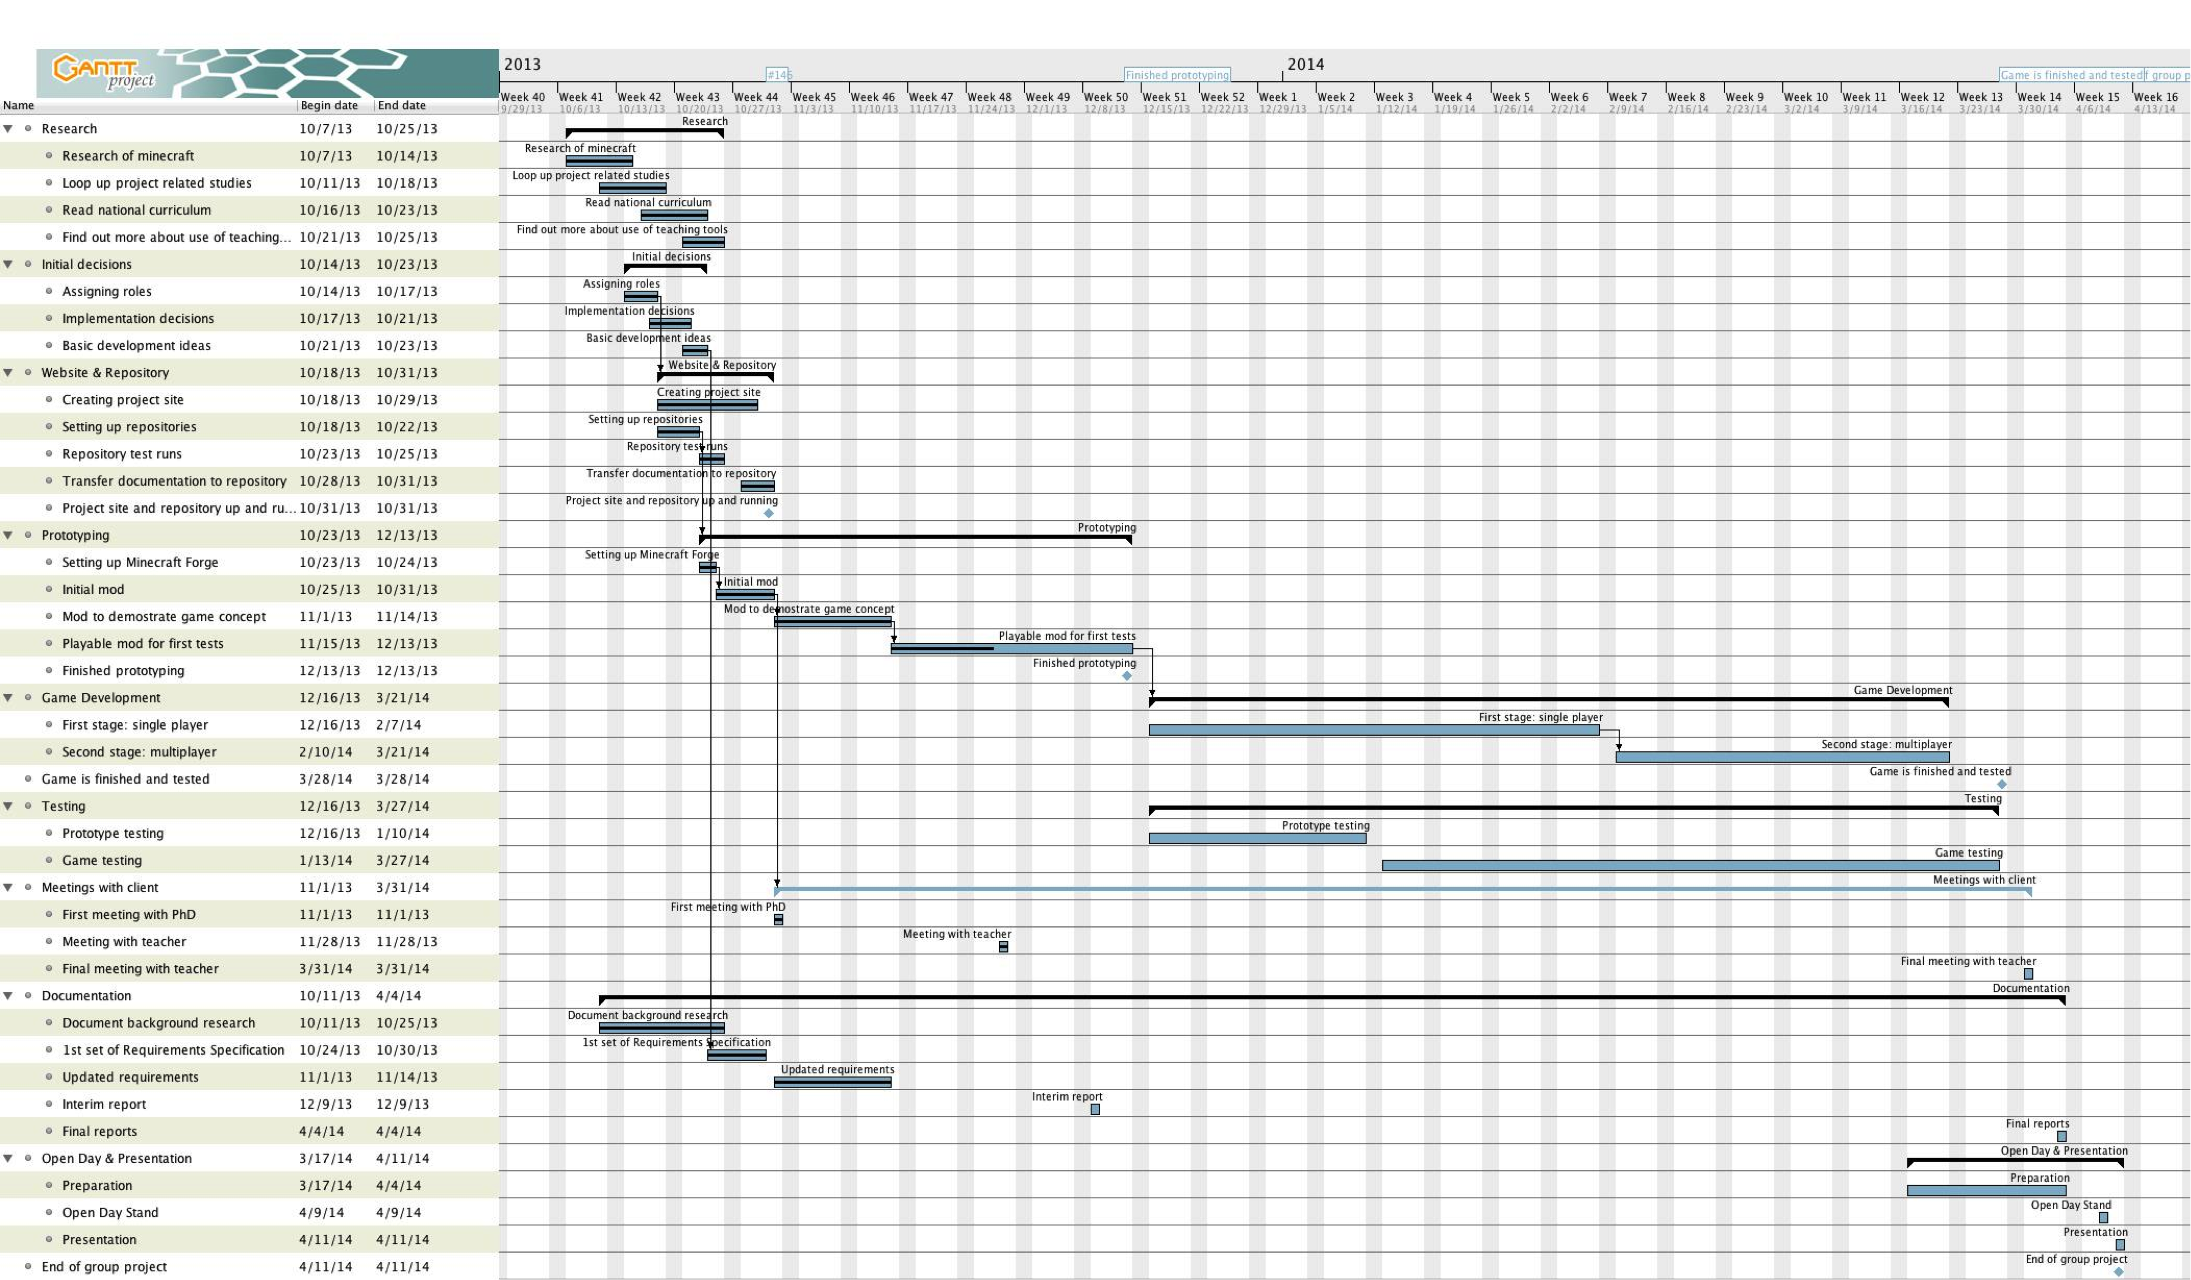
\includegraphics[width=24cm]{interim_gantt_chart}
\end{figure}
\end{landscape}